\documentclass[11pt, reqno]{amsart}

\usepackage[spanish]{babel}
\usepackage[LGR, T1]{fontenc}
\usepackage[utf8]{inputenc}

../LaTeX/general.tex
% \input{../graphics.tex}

\makeatletter
\def\emailaddrname{\textit{Correo electrónico}}
\def\subtitle#1{\gdef\@subtitle{#1}}
\def\@subtitle{}

% Metadata
\def\logo#1{\gdef\@logo{#1}}
\def\@logo{}
\def\institution#1{\gdef\@institution{#1}}
\def\@institution{}
\def\department#1{\gdef\@department{#1}}
\def\@department{}
\def\professor#1{\gdef\@professor{#1}}
\def\@professor{}
\def\course#1{\gdef\@course{#1}}
\def\@course{}
\def\coursecode#1{\gdef\@coursecode{#1}}
\def\@coursecode{}

\renewcommand{\maketitle}{
\begin{center}
	\small
	\renewcommand{\arraystretch}{1.2}
	\begin{tabular}{cp{.37\textwidth}p{0.44\textwidth}}
		% \hline
		\multirow{5}{*}{\includegraphics[height=2.0cm]{\@logo}}
	  & \multicolumn{2}{c}{ \makecell{{\bfseries \@institution} \\ \@department} } \\
	  % & \multicolumn{2}{c|}{{\bfseries\@institution} \\ \@department} \\
	  \cline{2-3}
	  & \textbf{Profesor:} \@professor & \textbf{Ayudante:} \authors \\
	  % \cline{2-3}
	  & \textbf{Curso:} \@course & \textbf{Sigla:} \@coursecode \\
	  % \cline{2-3}
	  & \multicolumn{2}{l}{ \textbf{Fecha:} \@date } \\
	  % \hline
	\end{tabular}
	\\[\baselineskip]
	% {}
	% \vspace{2\baselineskip}
	{\bfseries\Large\@title}
	\ifx\@subtitle\@empty\else
		\\[1ex]
		\large\mdseries\@subtitle
	\fi
\end{center}
}
\makeatother

\usepackage{multirow, makecell}

\usepackage[
	reversemp,
	letterpaper,
	% marginpar=2cm,
	% marginsep=1pt,
	margin=2.3cm
]{geometry}
\usepackage{fontawesome}
% \makeatletter
% \@reversemargintrue
% \makeatother

% Símbolos al margen, necesitan doble compilación
\newcommand{\hard}{\marginnote{\faFire}}
\newcommand{\hhard}{\marginnote{\faFire\faFire}}

% Dependencias para los teoremas
\usepackage{xifthen}
\def\@thmdep{}
\newcommand{\thmdep}[1]{
	\ifthenelse{\isempty{#1}}
	{\def\@thmdep{}}
	{\def\@thmdep{ (#1)}}
}
\newcommand{\thmstyle}{\color{thm}\sffamily\bfseries}

% ===== Estilos de Teoremas ==========
\newtheoremstyle{axiomstyle}
	{0.3cm}
	{0.3cm}
	{\normalfont}
	{0.5cm}
	{\bfseries\scshape}
	{:}
	{4pt}
	{\thmname{#1}\thmnote{ #3}\thmnumber{ (#2)}}
\newtheoremstyle{styleC}
	{0.5cm}
	{0.5cm}
	{\normalfont}
	{0.5cm}
	{\bfseries}
	{:}
	{4pt}
	{\thmname{#1\textrm{\@thmdep}}\thmnumber{ #2}\thmnote{ (#3)}}

% ====== Teoremas (sin borde) ===========
\theoremstyle{axiomstyle}
\newtheorem*{axiom}{Axioma}

% ====== Teoremas (sin borde) ==================
\theoremstyle{styleC}
\newtheorem{thm}{Teorema}[section]
\newtheorem{mydef}[thm]{Definición}
\newtheorem{prop}[thm]{Proposición}
\newtheorem{cor}[thm]{Corolario}
\newtheorem{lem}[thm]{Lema}
\newtheorem{con}[thm]{Conjetura}

\newtheorem*{prob}{Problema}
\newtheorem*{sol}{Solución}
\newtheorem*{obs}{Observación}
\newtheorem*{ex}{Ejemplo}

% \usepackage{tcolorbox}
% \newtcbox{bluebox}[1][]{enhanced jigsaw, 
%   sharp corners,
%   frame hidden,
%   nobeforeafter,
%   listing only,
%   #1} % comando para crear cajas de colores

\expandafter\let\expandafter\oldproof\csname\string\proof\endcsname
\let\oldendproof\endproof
\renewenvironment{proof}[1][\proofname]{%
  \oldproof[\scshape Demostración:]%
}{\oldendproof} % comando para redefinir la caja de la demostración
\newenvironment{hint}[1][\proofname]{%
  \oldproof[\scshape Pista:]%
}{\oldendproof} % comando para redefinir la caja de la demostración

% colores utilizados
\definecolor{numchap}{RGB}{249,133,29}
\definecolor{chap}{RGB}{6,129,204}
\definecolor{sec}{RGB}{204,0,0}
\definecolor{thm}{RGB}{106,176,240}
\definecolor{thmB}{RGB}{32,31,31}
\definecolor{part}{RGB}{212,66,66}

% ====== Diseño de los titulares ===============
\usepackage[explicit]{titlesec} % para personalizar el documento, la opción <<explicit>> hace que el texto de los titulares sea un objeto interactuable

\titleformat{\subsection}[runin]
	{\bfseries}
	{\textrm{\S}\thesubsection}
	{1ex}
	{#1.}

\setlist[enumerate,1]{label=\arabic*., ref=\arabic*} % Enumerate standards

% \usepackage{diagbox}

\title{Aún más aproximaciones}
\subtitle{Roth, Thue y ¿$abc$?}
\date{8 de septiembre de 2023}

\author[José Cuevas]{José Cuevas Barrientos}
\email{josecuevasbtos@uc.cl}

\logo{../puc_negro.png}
\institution{Pontificia Universidad Católica de Chile}
\department{Facultad de Matemáticas}
\course{Teoría de Números}
\coursecode{MAT2225}
\professor{Héctor Pastén}

\begin{document}

\maketitle

\section{El teorema de Roth y sus amigos}
\begin{thm}[Thue]
	Sea $f(x, y) \in \Z$ un polinomio homogéneo irreducible de grado $n := \deg f \ge 3$.
	Para todo entero $a \in \Z$ la ecuación diofántica $f(x, y) = a$ admite sólo finitas soluciones.
\end{thm}

\begin{enumerate}
	\item (Prueba de sanidad) Demuestre que se puede relajar un poco el teorema de Thue:
		
		Sea $f(x, y) \in \Z$ un polinomio homogéneo de grado $n := \deg f \ge 3$ que no es ni una potencia $n$-ésima de un polinomio lineal,
		ni la potencia $n/2$-ésima de un polinomio cuadrático.
		Para todo entero $a \ne 0$ la ecuación diofántica $f(x, y) = a$ admite sólo finitas soluciones.

		Discuta por qué las hipótesis son necesarias.

	\item \hard
		Sea $n > 0$ tal que $-1$ es un residuo cuadrático módulo $n$ (i.e., existe $r$ tal que $r^2 \equiv -1 \pmod n$).
		Emplee el teorema de aproximación de Dirichlet para demostrar que $n$ es suma de dos cuadrados.

		\begin{hint}
			La condición puede reescribirse como que $r^2 + 1^2 \equiv 0 \pmod n$ que es como decir que $n$ es (salvo un múltiplo)
			suma de dos cuadrados.
			El problema está en sacarse el múltiplo de encima, para lo que necesitas $a^2 + b^2 \equiv 0 \pmod n$ con $a, b$ <<chicos>>
			que es precisamente lo que los teoremas de aproximación pueden dar.
			% Será útil emplear dicho $r$.
			% Por lo demás, cuando $n \to \infty$ entonces $r/n \approx \sqrt{n^2 - 1}/n \approx 1$
		\end{hint}
\end{enumerate}

\begin{thm}[Roth, 1955]
	Sea $\alpha$ un real irracional algebraico.
	Para todo $\epsilon > 0$ la desigualdad
	$$ \left| \alpha - \frac{u}{v} \right| < \frac{1}{v^{2 + \epsilon}} $$
	admite sólo finitas soluciones.
\end{thm}

\begin{enumerate}[resume]
	\item Empleando el teorema de Roth, demuestre lo siguiente:

		Sea $f(x, y) \in \Z[x, y]$ un polinomio homogéneo de grado $d := \deg f$ sin factores lineales repetidos.
		Para todo $\epsilon > 0$ existe una constante $C := C_{f, \epsilon} > 0$ tal que si $n, m$ son coprimos entonces
		o bien $f(n, m) = 0$, o bien $|f(n, m)| \ge C |n|^{d - 2 - \epsilon}$
\end{enumerate}

\section{Cara B (de Bonus)}
\begin{enumerate}[resume]
	\item \textbf{Teorema de Kronecker:} sea $\alpha$ un real irracional.
		Demuestre que las partes fraccionarias $\{ n \alpha \}$ con $n\in\Z$ forman un subconjunto denso de $[0, 1)$.

		\begin{hint}
			Emplee algún tipo de argumento por principio del palomar, similar a la demostración del teorema de aproximación de Dirichlet.
		\end{hint}

	\item \hard
		(¿Jugamos al billar?)
		Considere el cuadrado $T := [0, 1] \times [0, 1]$ y tome un <<bola de billar>> $(x, y) \in T$ (donde $x, y \notin \{ 0, 1 \}$).
		Luego golpeamos la bola de billar con cierta pendiente $\alpha$.
		Asumiendo que la bola no pierde energía y rebota indefinidamente, el objetivo es demostrar lo siguiente:
		\begin{enumerate}
			\item Si $\alpha$ es racional, eventualmente la bola vuelve al punto de partida y, por tanto, hay puntos de la tabla para los cuales
				la bola jamás se acercará.%
				\footnote{Formalmente, existe un radio $\epsilon > 0$ tal que la bola jamás está a $<\epsilon$ del punto.}
			\item Si $\alpha$ es irracional demuestre que para todo punto $\vec p$ en la tabla la bola se acerca arbitrariamente a ellos;
				vale decir, que para todo $\epsilon > 0$ existe $t$ suficientemente grande tal que $\|(x(t), y(t)) - \vec p\| < \epsilon$.
		\end{enumerate}
\end{enumerate}

\section{Conjetura $abc$}
El resultado del ejercicio 3 parece contradictorio: o bien $f(n, m)$ es muy chico o es muy grande.
Resulta que no es nada contradictorio si cambiamos nuestro criterio de <<ser grande>> a <<tener muchos factores primos>>, lo que nos lleva a:
\begin{con}[$abc$ de Masser-Oesterlé]
	Para todo $\epsilon > 0$ existe una constante $\kappa_\epsilon > 0$ tal que para todo par $a, b$ de enteros coprimos positivos
	con $c := a + b$ se tiene que
	$$ c \le \kappa_\epsilon \left( \prod_{p \mid abc} p \right)^{1 + \epsilon}. $$
\end{con}

\begin{enumerate}[resume]
	\item \textbf{La conjetura de Catalan:} La ecuación $x^n - y^m = 1$ no admite soluciones con $x, y > 0$ y $n, m \ge 1$ además de $3^2 - 2^3 = 1$.

		Asumiendo la conjetura $abc$ demuestre que la conjetura de Catalan admite a lo sumo finitos contraejemplos.%
		\footnote{Ojo que estos finitos contraejemplos son en general, no para un exponente fijo.}

	\item \textbf{El Último Teorema de Fermat:} No existen $x, y, z > 0$ enteros con $n \ge 3$ tales que
		\[
			x^n + y^n = z^n.
		\]

		Asumiendo que conoce una demostración para los casos $n \in \{ 3, 4, 5 \}$ y asumiendo la conjetura $abc$
		demuestre que el Último Teorema de Fermat admite a lo sumo finitos contraejemplos.
\end{enumerate}

\section{Comentarios adicionales}
\begin{itemize}
	\item En el ejercicio 5 del billar, si en lugar de jugar en una mesa cuadrada, jugamos en una mesa circular, entonces el fenómeno es parecido pero no igual.
		Si golpeamos con pendiente irracional, la clausura de la trayectoria de la bola será ahora una corona o anillo (ver fig.~\ref{fig:billard_circle}).
		\begin{figure}[!hbt]
			\centering
			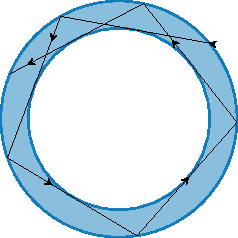
\includegraphics[scale=1]{../billard_circle.pdf}
			\caption{}%
			\label{fig:billard_circle}
		\end{figure}

		El lector interesado puede tratar de demostrar que éste es el caso (por ejemplo, es fácil demostrar que hay un círculo en donde la bola no entra
		y determinar el radio máximo de éste agujero) y recomendamos revisar el ejercicio 11.8.5 de
		\citeauthor{granville:masterclass}~\cite[422]{granville:masterclass}.

	\item No es coincidencia que la conjetura $abc$ <<trivialice>> el último teorema de Fermat (al menos asintóticamente).
		Relativamente podemos entender la conjetura $abc$ como una <<generalización>> de varios teoremas centrales en la teoría de números,
		como el último teorema de Fermat, el teorema de Faltings (o conjetura de Mordell), el teorema de Roth y el teorema de Baker.
		Para más información véase la nota de \citeauthor{granville2002abc}~\cite{granville2002abc}.

	\item Resultó altamente controversial al inicio de los 2000's el que el geómetra japonés Shinichi Mochizuki hubiese dado una <<demostración>>
		de la conjetura $abc$ mediante el uso de una teoría que él había desarrollado a lo largo de cientos de páginas.
		La situación ha sido peculiar desde el comienzo: Mochizuki se negó a publicar sus trabajos en revistas matemáticas, originalmente sólo dejándolas
		a disposición en japonés en su sitio web, pero más tarde ha traducido su trabajo al inglés.
		Más aún, el medallista Fields y numerista alemán Peter Scholze habría leído la obra de Mochizuki y declaraba encontrar un error irremediable
		en uno de sus corolarios; Mochizuki negó el criticismo de Scholze y publicó sus trabajos en una revista japonesa, tras lo cual el numerista
		Frank Calegari señala: <<Ahora tenemos la situación ridícula en la que $abc$ es un teorema en Kioto, pero una conjetura en el resto del mundo.>>
\end{itemize}

\nocite{granville:masterclass}
\printbibliography[title={Referencias y lecturas adicionales}]

\end{document}
